\begin{figure}[h]
    \centering
    \begin{minipage}[t]{0.48\textwidth}
        \centering
        \vspace{0pt}
        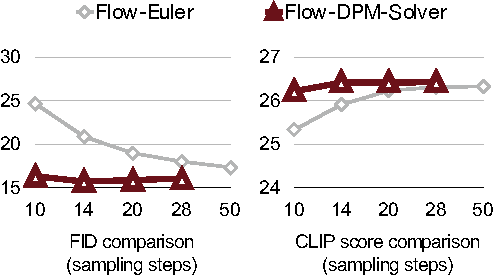
\includegraphics[width=1.0\linewidth]{figures/flow-sampler-ablation.pdf}
        \caption{Impact of sampling steps on FID and CLIP-Score: A Comparison between Flow-DPM-Solver and Flow-Euler.}
        \label{fig:flow_sampler_ablation}
    \end{minipage}
    \hfill
    \begin{minipage}[t]{0.48\textwidth}
        \centering
        \vspace{0pt}
        \captionof{table}{Comparison of different training schedules on 256$\times$256 resolution.}
        \label{tab:sampling_schedules}
        \vspace{-6pt}
        \scalebox{0.9}{
            \begin{tabular}{lccc}
                \toprule
                \textbf{Schedule} & \textbf{FID}~$\downarrow$ & \textbf{CLIP}~$\uparrow$ & \textbf{Iterations} \\
                \midrule
                DDPM & 19.5 & 24.6 & 120K \\
                Flow Matching & 16.9 & 25.7 & 120K \\
                \bottomrule
            \end{tabular}
        }
        
        \vspace{-5pt}
        \captionof{table}{Comparison of image-text pair sampling strategies during training.}
        \label{tab:dataset_clip_ablation}
        \vspace{2pt}
        \scalebox{0.9}{
            \begin{tabular}{lccc}
                \toprule
                \textbf{Prompt Strategy} & \textbf{FID}~$\downarrow$ & \textbf{CLIP}~$\uparrow$ & \textbf{Iterations} \\
                \midrule
                Single & 6.13 & 27.10 & 65K \\
                Multi-random & 6.15 & 27.13 & 65K \\
                Multi-clipscore & 6.12 & 27.26 & 65K \\
                \bottomrule
            \end{tabular}
        }
    \end{minipage}
\end{figure}